\section{Zielsetzung}
Im Versuch werden unbekannte Widerstände, Induktivitäten und Kapazitäten mittels
grundlegender Brückenschaltungen ermittelt.

\section{Theorie}
Brückenschaltungen kommen in der Messtechnik häufig zum Einsatz, da sie sehr genaue
Messergebnisse liefern.
Eine prinzipielle Brückenschaltung ist in \ref{Abb1} zu sehen.

\begin{figure}
  \centering
  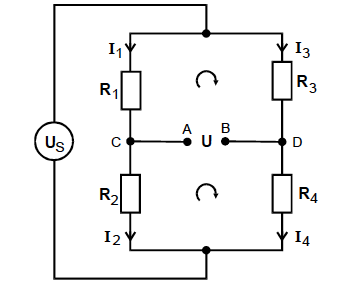
\includegraphics[scale=0.7]{Bruecke1.PNG}
  \caption{Abbildung einer prinzipiellen Brückenschaltung \cite{Quelle}}
  \label{Abb1}
\end{figure}
\FloatBarrier

\noindent Zwischen den beiden stromdurchflossenen Leitern wird an der Stelle A
und B in \ref{Abb1} eine Potentialdifferenz, die auch als Brückenspannung bezeichnet
wird, gemessen. Verschwindet diese Brückenspannung auf Grund entsprechend eingestellter
Widerstände $R_1 \symup{bis} R_4$, so wird die Brücke als abgeglichen bezeichnet.
Mittels der Kirchoff´schen Gesetze
\begin{align*}
  \sum{I_\symup{k}} &= 0 \\
  \sum{U_\symup{k}} &= 0
\end{align*}
ergeben sich folgende Bedingungen für Ströme und Spannung:
\begin{align*}
  I_1 = I_2 &\, I_3 = I_4 \\
  U = I_1 R_1 + I_3 R_3 &\, -U = -I_2 R_2 + I_4 R_4 .
  \end{align*}
  Diese Gleichungen und die Gleichung für die Speisespannung
\begin{align*}
  U_\symup{s} = I_1 (R_1 + R_2)
\end{align*}
ergeben folgenden Zusammenhang für die Brückenspannung $U$:
\begin{equation*}
  U = \frac{R_2 R_3 - R_1 R_4}{(R_3 + R_4)(R_1 + R_2)} U_\symup{s} .
\end{equation*}
Damit die Brückenschaltung als abgeglichen gilt, muss folglich gelten:
\begin{align}
  R_2 R_3 = R_1 R_4
\end{align}
Da dieser Zusammenhang lediglich vom Verhältnis der Widerstände zueinander und nicht
von $U_\symup{s}$ abhängig ist, kann damit leicht ein unbekannter Widerstand bestimmt
werden, solange die drei anderen bekannt sind.
Wenn in einer Brückenschaltung nicht nur Ohm´sche Widerstände verbaut sind, sondern
auch Kapazitäten und Induktivitäten, so werden Widerstände komplex dargestellt:
\begin{align*}
  X + iY = Z .
\end{align*}
Das macht aus Gleichung (1):
\begin{align*}
  Z_2 Z_3 = Z_1 Z_4
\end{align*}
Hierbei wird X als Wirkswiderstand und Y als Blindwiderstand bezeichnet. Auf Grund
der Tatsache, dass zwei komplexe Zahlen gleich sind, wenn deren Imaginär- und Realteil
gleich sind, muss folglich gelten:
\begin{align}
  X_2 X_3 - Y_2 Y_3 &= X_1 X_4 - Y_1 Y_4 \\
  X_1 Y_4 + X_4 Y_1 &= X_2 Y_3 + X_3 Y_2
\end{align}

\subsection{Wheatstone´sche Brückenschaltung}
Die Wheatstone´sche Brückenschaltung ist in \ref{Abb2} zu sehen und dient zur
Ermittlung den unbekannten Widerstandes $R_\symup{x}$. Hier sind ausschließlich Ohm´sche
Widerstände verbaut, weshalb die Schaltung sowohl mit Gleich- als auch mit
Wechselstrom betrieben werden kann, solange darauf geachtet wird, dass der Nullindikator
der Stromart entsprechend gewählt wird.

\begin{figure}
  \centering
  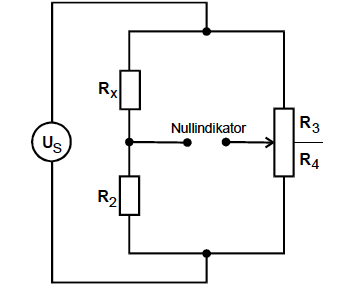
\includegraphics[scale=0.7]{Wheat.PNG}
  \caption{Wheatstone´sche Brückenschaltung \cite{Quelle}}
  \label{Abb2}
\end{figure}
\FloatBarrier

\noindent Da es hier lediglich auf das Verhältnis zwischen $R_3 / R_4$ ankommt, kann
an dieser Stelle ein Potentiometer verwendet werden.
Mit Hilfe von (1) ergibt sich folgende Formel für den unbekannte Widerstand
$R_\symup{x}$ :
\begin{align*}
  R_\symup{x} = R_2 \frac{R_3}{R_4} .
\end{align*}

\subsection{Kapazitätsmessbrücke}
Der komplexe Widerstand eines realen Kondensators ist:
\begin{align*}
  Z = R - \frac{i}{\omega C}
\end{align*}
Eine Brückenschaltung zur Bestimmung einer unbekannten Kapazität ist in \ref{Abb3}
zu sehen. Hier muss beachtet werden, dass sich hinter der unbekannten Kapazität
noch ein unbekannter Ohm´scher Widerstand befindet, der eine Phasenverschiebung
verursachen würde. Folglich müssen in der Schaltung zwei voneinander unabhängige
veränderliche Widerstände eingebaut werden. In der Graphik sind diese $R_2$ und das
Potentiometer für $R_3$ und $R_4$.
\FloatBarrier

\begin{figure}
  \centering
  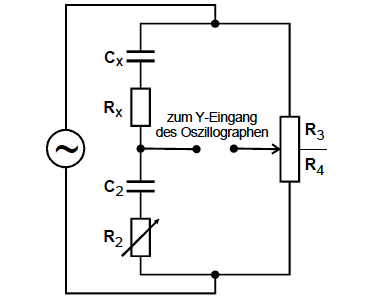
\includegraphics[scale=0.7]{Kapa.PNG}
  \caption{Kapazitätsmessbrücke \cite{Quelle}}
  \label{Abb3}
\end{figure}
Zum Bestimmen des unbekannten Widerstandes $R_\symup{x}$ und der unbekannten Kapazität
$C_\symup{x}$ gelten die Gleichungen:
\begin{align*}
  R_\symup{x} &= R_2 \frac{R_3}{R_4} \\
  C_\symup{x} &= C_2 \frac{R_4}{R_3} .
\end{align*}
\FloatBarrier

\subsection{Induktivitätsmessbrücke}
Der Aufbau einer Indutkivitätsmessbrücke ist analog zu dem der Kapzitätsmessbrücke. Ein
Teil der elektromagnetischen Feldenergie der Spule geht in Form von Wärme verloren.
Das Ersatzschaltbild einer solchen realen Induktivität ist eine ideale Induktivität
in Reihe geschaltet mit einem unbekannten Widerstand. Analog zur Messung der
unbekannten Kapazität, sind auch hier zwei voneinander unabhängig regelbare Widerstände
verbaut. Im Schaltbild \ref{Abb4} sind dies zum einen $R_2$ und zum anderen das
Potentiometer zur Bestimmung von $R_3$ und $R_4$. Der komplexe Widerstand einer realen
Spule ist:
\begin{align*}
  Z = R + i \omega L
\end{align*}
\begin{figure}
  \centering
  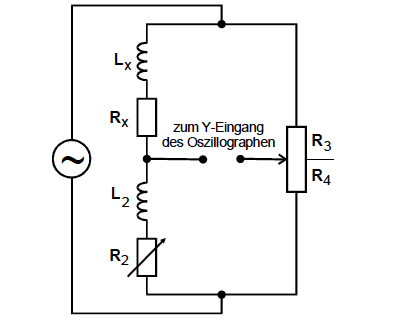
\includegraphics[scale=0.7]{Indu.PNG}
  \caption{Induktivitätsmessbrücke \cite{Quelle}}
  \label{Abb4}
\end{figure}
\FloatBarrier

\noindent Zur Bestimmung des unbekannten Widerstandes und der unbekannten Induktivität
gelten Folgende Gleichungen:
\begin{align*}
  R_\symup{x} &= R_2 \frac{R_3}{R_4} \\
  L_\symup{x} &= L_2 \frac{R_3}{R_4}
\end{align*}

\subsection{Maxwell-Brücke}
Die Maxwellbrücke stellt eine Alternative zur Bestimmung einer unbekannten Induktivität
dar. Die reale Induktivität wird auch hier wieder als Ersatzschaltung aus einer idealen
Induktivität und einem unbekannten Widerstand, die in Reihe geschaltet sind dargestellt.
Im Unterschied zur Induktivitätsmessbrücke ist hier anstelle der zweiten bekannten Induktivität
eine möglichst verlustarme Kapazität $C_4$ parallel zu $R_2$ geschaltet.
\begin{figure}
  \centering
  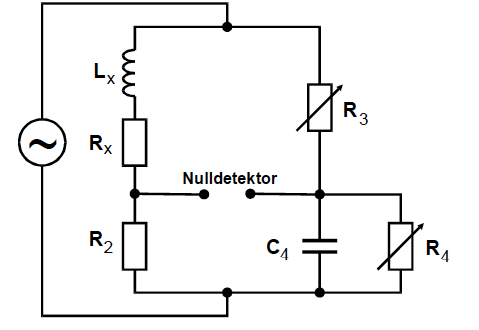
\includegraphics[scale=0.7]{Max.PNG}
  \caption{Maxwellbrückenschaltung zur Bestimmung einer unbekannten Induktivität \cite{Quelle}}
  \label{Abb5}
\end{figure}
\FloatBarrier
Für den Widerstand der unbekannten Induktivität gilt:
\begin{align*}
  Z_\symup{x} = R_\symup{x} + i \omega L_\symup{x} \frac{1}{Z_4} .
\end{align*}
Des weiteren gilt für die eingebaute Kapazität $C_4$ :
\begin{align*}
  \frac{1}{Z_4} = \frac{1}{R_4} + i \omega C_4 .
\end{align*}
Nun müssen zur Bestimmung des unbekannten Widerstandes und der unbekannten Indutkivität
die komplexen Abgleichbedingungen (2) und (3) beachtet werden:
\begin{align*}
  R_\symup{x} &= R_2 \frac{R_3}{R_4} \symup{und} \\
  L_{x} &= R_2 R_3 C_4
\end{align*}
\subsection{Wien-Robinson-Brücke}
Die Wien-Robinson-Brücke ist im Gegensatz zu den zuvor beschriebenen Brücken
frequenzabhängig. In \ref{Abb6} ist eine solche Brückenschaltung dargestellt.
\begin{figure}
  \centering
  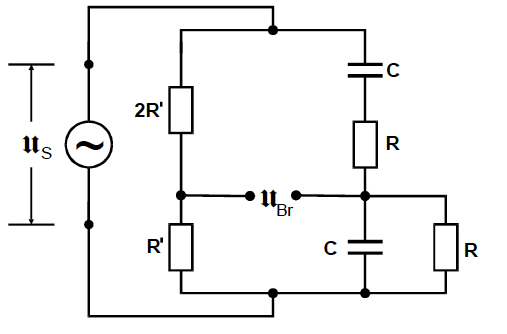
\includegraphics[scale=0.7]{Wien.PNG}
  \caption{Schaltbild einer Wien-Robinson-Brücke \cite{Quele}}
  \label{Abb6}
\end{figure}
In der Schaltung werden keine Abgleichelemente verbaut. Hier wird das Verhältnis
der Brückenspannung zur Speisespannung betrachtet, für welches folgende Gleichung
gilt:
\begin{align*}
  \left|\frac{U_\symup{Br}}{U_\symup{s}} \right|^2 = \frac{\left(1 - (\omega R C)^2\right)^2}{9 \left( 1 - (\omega R C)^2\right)^2 + 81(\omega R C)^2}
\end{align*}
An der Formel lässt sich erkennen, dass die Brückenspannung bei $\omega_0 = \frac{1}{RC}$
verschwindet und die Brücke damit abgeglichen ist.
Die Wien-Robinson-Brücke dient als Frequnezfilter, was aus der obigen Gleichung nicht
direkt zu erkennen ist. Wird in dieses Verhältnis $\Omega := \frac{\omega}{\omega_0}$
eingebracht, so ist die Frequenzfiltereigenschaft der Brücke deutlch zu erkennen:
\begin{align*}
  \left|\frac{U_\symup{Br}}{U_\symup{s}} \right|^2 = \frac{1}{9} \frac{\left(1 - \Omega^2\right)^2}{\left(1 - \Omega^2\right)^2 + 9\Omega^2}
\end{align*}

\section{Durchführung}
Zur Durchführung des Versuchs werden die in der Theorie beschriebenen Brückenschaltungen,
ein Oszilloskop zur Messung der Brückenspannung, sowie ein Funktionengenerator, der die
Brückenschaltungen mit einer Sinusspannung versorgt, benötigt.

\subsection{Wheatstonebrücke}
Mit Hilfe der Wheatstonebrücke werden die unbekannten Widerstände "Wert 14" und "Wert 12"
bestimmt. Für das Verhältnis zwischen $R_3 \symup{und} R_4$ wird ein Potentiometer verwendet.
Es werden drei Messungen durchgeführt, mit jeweils unterschiedlichem $R_2$, um den Fehler
zu bestimmen. Bei jeder der Messungen gilt es, das Potentiometer so einzustellen, dass auf dem
Oszilloskop eine Nullinie zu erkennen ist.

\subsection{Kapazitätsmessbrücke}
Mit der kapazitätsmessbrücke werden verschiedene unterschiedliche Kapazitäten "Wert 13",
"Wert 1" und "Wert 8" bestimmt. Das Vorgehen zur Fehlerermittlung erfolgt analog zur
Wheatstonebrücke, es werden drei Messungen, mit jeweils unterschiedlicher Kapazität
$C_2$ durchgeführt, bei denen das Potentiometer stets so eingestellt wird, dass im
Oszilloskop eine Nullinie zu erkennen ist. Zu beachten ist, dass zur Bestimmung verlustbehafteter
Kapazitäten, ein variabler Widerstand $R_2$ verwendet werden muss, der alternierend
mit dem Potentiometer für $R_3 \symup{und} R_4$ verändert wird, um auf dem Oszilloskop
die Nullinie zu erzeugen.

\subsection{Induktivitätsmessbrücke}
Die Induktivitätsmessbrücke wird verwendet, um die verlustbehaftete Spule "Wert 17" zu bestimmen.
Auch hier ist $R_2$ ein regelbarer Widerstand und für $R_3 \symup{und} R_4$
wird ein Potentiometer verwendet. Wieder wird sich der Darstellung der Nullinie
auf dem Oszilloskop angenähert, indem $R_2$ und das Potentiometer alternierend geändert werden.

\subsection{Maxwell-Brücke}
Um die Maxwell-Brücke mit der Induktivitätsmessbrücke vergleichen zu können, wird anschließend
"Wert 17" noch einmal mit der Maxwell-Brücke bestimmt. Hier wird ein fixer Widerstand $R_2$
für drei unterschiedliche Messungen variiert, um den Fehler bei der messung zu ermitteln. Das
Potentiometer für $R_3 \symup{und} R_4$ bleibt auch hier bestehen.

\subsection{Wien-Robinson-Brücke}
Mit der Wien-Robinson-Brücke wird die Frequenzabhänhgigkeit der Brückenspannung untersucht.
Dafür wird die Frequenz der Speisespannung für 30 Werte zwischen \SI{20}{\Hz} und \SI{30}{\kilo\Hz}
variiert und die Brückenspannung abgelesen. Hierfür ist es sinnvoll, zunächst $\omega_0$ zu
ermitteln, um in diesem Bereich mehrere kleine Frequenzänderungen vorzunehmen.
Mit Hilfe der gemessenen Werte wird schließlich der Klirrfaktor bestimmt, welcher ein Maß für
die Qualität der Sinusschwingung ist.


\section{Auswertung}
Im folgenden werden vermehrt Mittelwerte und Standardabweichungen berechnet, hierfür werden folgenden Formeln verwendet:

\begin{equation}
  \bar{x} = \frac{1}{n} \sum{x_n}
  \label{Mittelwert}
\end{equation}

\begin{equation}
\upsigma = \frac{1}{\sqrt{n}} \sqrt{\frac{\sum{(x_n - \bar{x})^2}}{n-1} }
\label{Standardabweichung}
\end{equation}

Die Toleranz der Werte für $R_2$ , $C_2$ und $L_2$ wird vom Hersteller mit \SI{0.2}{\%} beschrieben.
\subsection{Wheatstonesche Brücke}
Der Bruch $\frac{R_3}{R_4} $ist mit einem Fehler von \SI{0.3}{\%} behaftet.
Die Messwerte für die Rechnung für $R_x$ und $\Delta R_x$ sind in der Tabelle \ref{tab:1} aufgelistet und werden somit durch

\begin{equation}
  \label{Widerstand}
  R_x = R_2 \frac{R_3}{R_4}
\end{equation}
und
\begin{equation}
  \label{FehlerWiderstand}
  \Delta R_x = \sqrt{\left(\frac{R_3}{R_4} \cdot 0.002 R_2\right)^2 + \left(R_2 \cdot 0.005 \frac{R_3}{R_4}\right)^2}
\end{equation}

berechnet.

\begin{table}
  \centering
  \caption{Messwerte Wheatstonebrücke.}
  \label{tab:1}
  \begin{tabular}{c c c c c}
    \toprule
    $R_2$ / \si{\ohm} & $R_3$ / \si{\ohm} & $R_4$ / \si{\ohm} & $R_x$ / \si{\ohm} & $\Delta R_x$ / \si{\ohm}\\
    \midrule
    Wert 14 & & &  &\\
    \midrule
    1000 & 473 & 527 & 897.53 & \pm 4.83\\
    664 & 576 & 423 & 904.17 & \pm 4.87\\
    332 & 732 & 268 & 906.81 & \pm 4.88 \\
    \midrule
    Wert 12 & & & & \\
    \midrule
    332 & 541 & 459 & 391.31 & \pm 2.11 \\
    1000 & 279 & 721 & 386.96 & \pm 2.08 \\
    664 & 369 & 631 & 388.30 & \pm 2.09 \\
    \bottomrule
  \end{tabular}
\end{table}

Daraus folgt mit \eqref{Mittelwert} und \eqref{Standardabweichung}

\begin{align*}
  \bar{R}_{\symup{Wert14}} &= \SI{902.84(478)}{\ohm} \\
  \bar{R}_{\symup{Wert12}} &= \SI{388.86(223)}{\ohm} \, .
\end{align*}

\subsection{Kapazitätsmessbrücke}
Erneut wird hier der Fehler von $\frac{R_3}{R_4}$ mit \SI{0.3}{\%} und der Fehler von $R_2$ mit \SI{3}{\%} angegeben.
Die gemessenen Werte zur Bestimmung der Kapazität eines Kondensators sind in Tabelle \ref{tab:2} aufgelistet.
Die Kapazität des Kondensators wird mit den Formeln

\begin{equation}
  \label{Kapazität}
  C_x = C_2 \frac{R_4}{R_3}
\end{equation}
und
\begin{equation}
  \label{FehlerKapazität}
  \Delta C_x = \sqrt{\left(\frac{R_3}{R_4} \cdot 0.002 C_2\right)^2 + \left(C_2 \cdot 0.005 \frac{R_3}{R_4}\right)^2}
\end{equation}
berechnet.

\begin{table}
  \centering
  \caption{Messwerte zur Bestimmung der Kapazität eines Kondensators.}
  \label{tab:2}
  \begin{tabular}{c c c c c}
    \toprule
    $C_2$ / \si{\nano\farad} & $R_3$ / \si{\ohm} & $R_4$ / \si{\ohm} & $C_x$ / \si{\nano\farad} & $\Delta C_x$ / \si{\nano\farad}  \\
    \midrule
    Wert 13 & & & &\\
    \midrule
    750 & 639 & 361 & 432.71 & \pm 2.33 \\
    994 & 703 & 297 & 419.94 & \pm 2.26 \\
    450 & 517 & 483 & 420.41 & \pm 2.26 \\
    \midrule
    Wert 1 & & & & \\
    \midrule
    450 & 405 & 595 & 661.11 & \pm 3.56 \\
    994 & 601 & 399 & 659.91 & \pm 3.55 \\
    750 & 529 & 471 & 667.77 & \pm 3.60 \\
    \bottomrule
  \end{tabular}
\end{table}

Daraus folgt mit \eqref{Mittelwert} und \eqref{Standardabweichung}

\begin{align*}
  \bar{C}_{\symup{Wert13}} &= \SI{421.35(145)}{\nano\farad} \\
  \bar{C}_{\symup{Wert1}} &= \SI{662.93(299)}{\nano\farad} \, .
\end{align*}


Für die Bestimmung einer RC-Kombination wurden die Werte aus Tabelle \ref{tab:3} gemessen und mit \eqref{Widerstand}, \eqref{FehlerWiderstand},
\eqref{Kapazität} und \eqref{FehlerKapazität} bestimmt.

\begin{table}
  \centering
  \caption{Messwerte zur Bestimmung einer RC-Kombination.}
  \label{tab:3}
  \begin{tabular}{c c c c c c c c}
    \toprule
    $C_2$ / \si{\nano\farad} & $R_2$ / \si{\ohm} & $R_3$ / \si{\ohm} & R$_4$ / \si{\ohm} &  $R_x$ / \si{\ohm} & $\Delta R_x$ / \si{\ohm} &
    $C_x$ / \si{\nano\farad} & $\Delta C_x$ / \si{\nano\farad} \\
    \midrule
    Wert 8 & & & & & & & \\
    \midrule
    450 & 380 & 604 & 396 & 579.60 & \pm 3.12 & 295.03 & \pm 1.58 \\
    994 & 172 & 771 & 229 & 579.10 & \pm 3.12 & 295.23 & \pm 1.59 \\
    750 & 230 & 716 & 284 & 579.86 & \pm 3.12 & 297.49 & \pm 1.60 \\
    \bottomrule
  \end{tabular}
\end{table}

Daraus folgt mit \eqref{Mittelwert} und \eqref{Standardabweichung}

\begin{align*}
  \bar{R}_{\symup{Wert8}} &= \SI{579.52(28)}{\ohm} \\
  \bar{C}_{\symup{Wert8}} &= \SI{295.91(97)}{\nano\farad} \, .
\end{align*}

\subsection{Induktionsmessbrücke}
Die Fehler von $R_3$ und $R_4$ werden mit \SI{3}{\%} angegeben.
Die Messwerte für die Rechnung für $L_x$ sind in der Tabelle \ref{tab:4} aufgelistet und werden mit \eqref{Widerstand}, \eqref{FehlerWiderstand} und

\begin{equation}
  \label{Induktivität}
  L_x = L_2 \frac{R_3}{R_4}
\end{equation}

\begin{equation}
  \label{FehlerInduktivität}
  \Delta L_x = \sqrt{\left(\frac{R_3}{R_4} \cdot 0.002 L_2\right)^2 + \left(L_2 \cdot 0.005 \frac{R_3}{R_4}\right)^2}
\end{equation}

berechnet.

\begin{table}
  \centering
  \caption{Messwerte für die Bestimmung einer LC-Kombination durch die Induk- tionsmessbrücke.}
  \label{tab:4}
  \begin{tabular}{c c c c}
    \toprule
    $L_2$ / \si{\milli\henry} & $R_2$ / \si{\ohm} & $R_3$ / \si{\ohm} & $R_4$ / \si{\ohm} \\
    \midrule
    Wert 17 & & & \\
    \midrule
    14.6 & 34 & 743 & 257 \\
    \bottomrule
  \end{tabular}
\end{table}

\begin{align*}
  R_x &= \SI{98.30(52)}{\ohm} \\
  L_x &= \SI{42.21(23)}{\milli\henry}
\end{align*}

\subsection{Maxwellbrücke}
Die Berechnung der LC-Kombination wird erneut mit der Maxwellbrücke durchgeführt. Die Messwerte sind in \ref{tab:5} aufgelistet und
$R_x$ und $L_x$ werden mit \eqref{Widerstand}, \eqref{FehlerWiderstand} und

\begin{align*}
  L_x &= R_2 R_3 C_4 \\
  \Delta L_x &= \sqrt{(0.002R_2 \cdot R_3 R_4)^2 + (0.03R_3 \cdot R_2 R_4)^2 +(0.03R_4 \cdot R_2 R_3)^2}
\end{align*}
berechnet.

\begin{table}
  \centering
  \caption{Messwerte für die Bestimmung einer LC-Kombination durch die Maxwellbrücke.}
  \label{tab:5}
  \begin{tabular}{c c c c}
    \toprule
    $C_4$ / \si{\nano\farad} & $R_2$ / \si{\ohm} & $R_3$ / \si{\ohm} & R$_4$ / \si{\ohm}  \\
    \midrule
    Wert 17 & & & \\
    \midrule
    750 & 664 & 84 & 632 \\
    \bottomrule
  \end{tabular}
\end{table}

\begin{align*}
  R_x &= \SI{88.25(48)}{\ohm} \\
  L_x &= \SI{41.83(178)}{\milli\henry}
\end{align*}

\subsection{Wien-Robinson-Brücke}
Die Kapazitäten, Induktivitäten und Widerstande der verwendeten Bauteile stehen in Tabelle \ref{tab:6}.

\begin{table}
  \centering
  \caption{Bauteilgrößen.}
  \label{tab:6}
  \begin{tabular}{ccc}
    \toprule
    $R'$ / \si{\ohm} & $R$ / \si{\ohm} & $\bar{C}_\symup{Wert1}$ / \si{\nano\farad} \\
    \midrule
    332 & 1000 & 662.93 \\
    \bottomrule
  \end{tabular}
\end{table}

Die gemessenen Werte für die Frequenzabhängigkeit der Brückenspannung der Wien-Robinson-Brücke sind in Tabelle \ref{tab:7} aufgelistet.

\begin{table}
  \centering
  \caption{Frequenzabhängikeit der Brückenspannung (Wien-Robinson-Brücke).}
  \label{tab:7}
  \begin{tabular}{c c}
    \toprule
    $\nu$ / \si{\hertz} & $U_B$ / \si{\milli\volt}\\
    \midrule
    20  & 648  \\
    40  & 608  \\
    60  & 536  \\
    80  & 456  \\
    100 & 392  \\
    130 & 288  \\
    160 & 184  \\
    190 & 104  \\
    220 & 40  \\
    240 & 2  \\
    260 & 34  \\
    280 & 67  \\
    310 & 110  \\
    350 & 162  \\
    400 & 220  \\
    500 & 305  \\
    800 & 472  \\
    1200  & 552  \\
    1600  & 600  \\
    4000  & 632  \\
    7000  & 624  \\
    9000  & 616  \\
    11000 & 608  \\
    15000 & 560  \\
    19000 & 504  \\
    23000 & 440  \\
    26000 & 392  \\
    30000 & 344  \\
    \bottomrule
  \end{tabular}
\end{table}

Die Werte aus Tabelle \ref{tab:6} werden im Diagramm \ref{fig:1} eingetragen und es wird eine Regression der Form
\begin{equation*}
   \left|\frac{U_B}{U_S}\right| = \sqrt{\frac{1}{9} \frac{(a^2 - 1)^2}{(1-a^2)^2 + 9 a^2}}
  \end{equation*}
durchgeführt, mit

\begin{align*}
  a &= \frac{\nu}{\nu_0} \\
  \nu_0 &= \frac{1}{RC \, 2\pi} \approx \SI{240.08}{\hertz}\\
  U_0 &= \SI{2.12}{\volt} \, .
\end{align*}

\begin{figure}
  \centering
  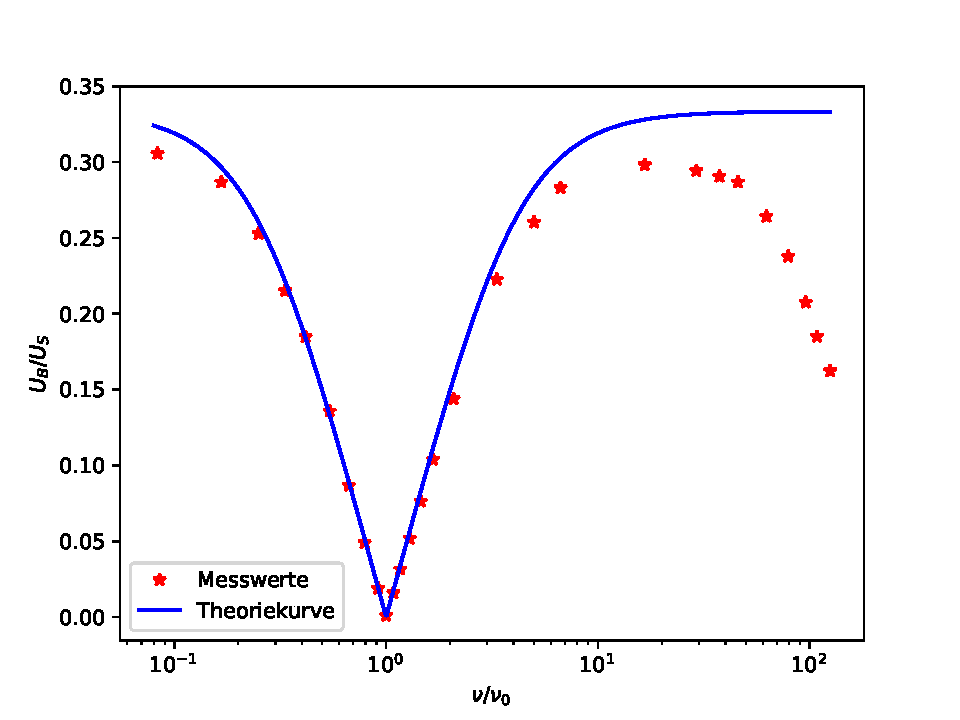
\includegraphics[scale=0.7]{plotFrequenz.pdf}
  \caption{Frequenzabhängigkeit der Brückenspannung (Wien-Robinson-Brücke).}
  \label{fig:1}
\end{figure}

\subsection{Klirrfaktor}
Im letzten Teil des Versuchs soll der Klirrfaktor bestimmt werden. Hierzu wird näherungsweise davon ausgegangen,
dass nur die 2. Oberwelle für den Klirrfaktor relevant ist.
Zunächst muss die Amplitude der 1. Oberwelle ausgerechnet werden, mit

\begin{equation*}
  U_2 = \frac{U_B}{\sqrt{\frac{(2^2 -1)^2}{9 [(1-2^2)^2 + 9 \cdot 2^2]}}} \approx \SI{0.738}{\volt}
\end{equation*}

Und somit folgt für den Klirrfaktor

\begin{equation*}
  k = \frac{U_2}{U_1} \approx 0.348 .
\end{equation*}

\section{Diskussion}
Da keine Theorie- bzw. Vergleichswerte angegeben sind, kann nur vermutet werden, dass die Werte, aufgrund des geringen Fehlers, realtiv genau
gemessen wurden.
Bei der Messung der Induktivität (Induktivitätsbrücke, Maxwell-Brücke) kann nur eine Messung durchgeführt werden, da das Abgleichen mit
dem Potentiometer nicht möglich war, da keine Nulllinie auf dem Oszilloskop sichtbar gemacht werden konnte. Dies könnte darauf hindeuten, dass
die zweite bekannte Spule in der Induktivitätsmessbrücke und die Kapazität in der Maxwell-Brücke verlustbehaftete Größen waren und nicht,
wie im Aufbau gefordert, verlustarm.
Zu erkennen ist, dass die Theoriekurve in höheren Frequenzen nicht nach unten abweicht, im gegensatz zu unseren Messwerten.
Das lässt sich damit erklären, dass der eingebaute Kondensator bei höheren Frequenzen blockiert, er kann sich also nicht mehr
schnell genug auf- und endladen.



\nocite{*}
\printbibliography
